\documentclass[11pt,reqno]{amsart}
\usepackage[top=1in, left=1in, right=1in, bottom=1in]{geometry}                % See geometry.pdf to learn the layout options. There are lots.
\geometry{letterpaper}                   % ... or a4paper or a5paper or ...
\usepackage[parfill]{parskip}    % Activate to begin paragraphs with an empty line rather than an indent
%\usepackage{algorithm, algorithmic}

\usepackage{algorithm}
\usepackage{algpseudocode}

\usepackage{graphicx}

\usepackage{verbatim}
\usepackage{amssymb}
\usepackage{amsmath}

\usepackage{enumitem}

\usepackage{setspace}
\doublespacing

\usepackage{natbib}

%\usepackage{epstopdf}
%\DeclareGraphicsRule{.tif}{png}{.png}{`convert #1 `dirname #1`/`basename #1 .tif`.png}

\newcommand{\RR}{I\!\!R} %real numbers
\DeclareMathOperator{\diag}{diag}

\algnewcommand{\Inputs}[1]{%
  \State \textbf{Inputs:}
  \Statex \hspace*{\algorithmicindent}\parbox[t]{.8\linewidth}{\raggedright #1}
}
\algnewcommand{\Initialize}[1]{%
  \State \textbf{Initialize:}
  \Statex \hspace*{\algorithmicindent}\parbox[t]{.8\linewidth}{\raggedright #1}
}

\title[RVD3]{Variant detection model with improved robustness and accuracy for low-depth targeted next-generation sequencing data}
\author{}
%\date{}                                           % Activate to display a given date or no date

\begin{document}

\begin{abstract}
%Massively parallel sequencing data has been generated by next-generation sequencing (NGS) technology for single nucleotide variants (SNVs) identification among related populations.
%To address the detection of SNVs, a variety of methods are being under-represented.
%However, by the reason of the error rate of the clonal heterogeneity and the limitation of the algorithms, identifying the true variants at minor allele frequencies for the very low sequencing read depth remains challenging.

%We propose a novel empirical Bayesian model to call variants in heterogeneous samples accurately. We present a Bayeisan sensitivity analysis of this hierarchical model to variations of the prior function.
%Our model with information prior (log-normal prior) and non-information prior (Jeffreys prior) both performs a high accuracy (96\%) when applied to a known 0.1\% minor allele frequency within very low read depth (39).
%Moreover, the model with Jeffreys prior presents much lower false discovery rate (FDR) to a known 0.1\% minor allele frequency event, compared with using improper prior.
%For further validation, our statistical model was applied on the yeast sequence data which also shows a high specificity and sensitivity over a wide range of read depth.
%This model is able to detect the emergence of a beneficial SNV earlier than was previously shown.
%Variant detection model with improved robustness and accuracy for low-depth targeted next-generation sequencing data

% The same with the Abstract poster of RECOMB2014.
Massively parallel sequencing data generated by next-generation sequencing (NGS) technology is routinely used to detect single nucleotide variants (SNVs) in research samples.
An emerging challenge for this technology is the identification of SNVs in heterogeneous cell populations with low read-depth data.
We have developed a Bayesian statistical model is able to share information between correlated positions and call low-frequency variants in heterogeneous samples.
We present a Bayesian sensitivity analysis of the model to variations in the prior function.
Our model with different priors both performs a high accuracy, and a Jeffrey's prior gives a lower false discovery rate (FDR) to detect a 0.1\% minor allele frequency event within minor read depth compared with an improper prior.
In an analysis of a directed evolution experiment, we are able to detect the emergence of a beneficial SNV earlier than was previously shown.

\end{abstract}

\maketitle

%%%%%%%%%%%%%%%%%%
% Introduction
%%%%%%%%%%%%%%%%%%
\section{Introduction}

Massively parallel sequencing data has been generated by Next-generation sequencing (NGS) technology to benefit clinical diagnostics and sequencing based phylogenetic analyses.
One primary application of NGS is variation detection among related populations and separate novel single-nucleotide variants (SNVs) candidates.
Somatic SNVs are detected by comparing the tumor and corresponding normal samples.

To address the detection of SNVs at low allele frequencies, a number of algorithms from NGS platform are being under-represented.
Strelka \citep{Saunders:2012fh}, VarScan2 \citep{Koboldt:2012cga}, JointSNVMix \citep{roth2012jointsnvmix} are highly used to differentiate somatic SNVs from germline cells.
Also, SAMtools \citep{li2009sequence}, Genome Analysis Toolkit (GATK) \citep{McKenna:2010bva}, and MuTect \citep{Cibulskis:2013ta} broadly concentrate on detecting low-frequency variants.
Through the comparision of these somatic mutation callers \citep{wang2013detecting}, VarScan2 excelled at the detection of high coverage and allele frequecy, while MuTect outperformed the other methods in detecting the low allelic fraction SNVs.
However identifying the true SNVs remains challenging because of the high false positive rate or high false negative rate which are mainly caused by the clonal heterogeneity.

Recently empirical Bayesian approaches have been made use to identify SNVs, which can automatically adjust for multiple testing and selection bias \citep{liao2014prior}.
A empirical Bayesian framework for somatic mutation detection from cancer genome sequencing data - EBCall, enables accurate mutations calling with low allele frequencies (less than 10\%) in a minor tumour subpopulation \citep{shiraishi2013empirical}.
Another method based on empirical Bayesian hierarchical model - RVD, was proposed for ultrasensitive rare SNV detection using beta-binomial model \citep{Flaherty:2011ja}.
RVD method is demonstrated to robustly detect mutations at 0.1\% fractional representation, which means accurately call one mutant per every 1000 wild-type alleles.
With the shortcoming of high read depth estimation in RVD, we originally built an improved robustness and accuracy model - RVD3 for low-depth SNVs detection.
Variants calling ability is tested and analyzed both on the synthetic sequence data and the true yeast sequencing data with different read depths.

In this article, RVD3 model - a novel Bayesian structure to accurately identify SNVs with small false discovery rate is first described in detail.
Secondly, Metropolis-within-Gibbs sampling is evolved for inference. And then to detect variants, a Bayesian posterior distribution is taken for hypothesis test.
Furthermore, we analyze the sensitivity of the Bayesian model to different priors - Jeffrey's prior, log-normal prior, and improper prior.
Finally, we choose Jeffrey's prior for the RVD3 model and demonstrate its performance on the yeast sequence data.
Thus our Bayesian model achieves a enhanced robustness and accuracy when calling variants for the low read depth and minor allele frequencies.

%%%%%%%%%%%%%%%%%%
% Data Sets
%%%%%%%%%%%%%%%%%%
\section{Data Sets}

\subsection{Synthetic DNA Sequence Data}

Two 400bp DNA sequences(control/case) were synthesized with only 14 different single nucleotide positions. Sample of the case and control DNA were mixed to yield 0.1\%, 0.3\%, 1\%, 10\%, and 100\% defined minor allele frequencies (MAFs).
The details of the experimental protocol are available from the original publication~\citep{Flaherty:2011ja}.
We used BWA v0.7.5a to align the short sequencing reads to the reference sequence. The -C50 option of BWA was taken to remove the reads of low mapping quality.
BAM files were sampled by $10\times$, $100\times$, $1,000\times$, and $10,000\times$ using Picard v1.104 (http://picard.sourceforge.net).
The final data set contains read pairs for $N=6$ replicates for the control at different MAF levels.

\subsection{Yeast Data}
We first mapped the wild-tpye strain GSY1135 \citep{kvitek2011reciprocal} to Chromosome 10 in S288c reference genome (SGD; http://www.yeastgenome.org/) by BWA v0.7.5a \citep{li2009fast}.
Then called SNPs by GATK v2.5 UnifiedGenotyper \citep{McKenna:2010bva, depristo2011framework} and created a FASTA GSY1135 reference using GATK FastaAlternative.
Secondly, we downloaded generation 7 as control and generation 133 as case in experiment 1 from \citep{kvitek2013whole}, and removed WT population using FASTX Barcode Splitter and cut down the pair ends accordingly.
The FASTQ files of case and control were mapped to the corresponding reference genome created before.
Then wen used SAMtools v0.1.19 \citep{li2009sequence} to convert the alignment files to the binary alignment map (BAM) format.
Next, pileup files were generated by SAMtools and depth chart file were derived for further SNVs detection.

%%%%%%%%%%%%%%%%%%
% RVD3 Model
%%%%%%%%%%%%%%%%%%
\section{RVD3 Model}

\subsection{Model Structure}\label{sec:model_structure}
RVD is based on a two-stage hierarchical Bayesian model for variant detection \citep{Flaherty:2011ja}. Through hypothesis test on case and control samples by RVD, we can call the variants successfully.
Now RVD3 has three-stage model including priors built on the former RVD model.
The definitions for sample data are given: $r_{ji}$ is the number of reads with a non-reference base at position $j$ in replicate $i$, and $n_{ji}$ is the total number of reads at position $j$ in replicate $i$.
Three parameters of the model are: $\mu_0$, a global error rate; $M_0$, the global position which estimates the variation in the error rate across the positions;
to choose a priori distribution for $M_j$, log-normal prior and Jeffrey's prior \citep{jeffreys1946invariant} are employed, which enhances the former RVD model \citep{Flaherty:2011ja}.
Here $M_j$ is the local precision measures the alteration in the error rate across replicates at position $j$. The graphical chart for RVD3 is shown in Figure~\ref{fig:graphical_model}.

RVD3 hierarchically includes three levels of samplings: $r_{ji} | n_{ji} \thicksim \text{Binomial}(\theta_{ji}, n_{ji})$ models the variation due to sampling the pool of DNA molecules on the sequencer.
$\theta_{ji} \thicksim \text{Beta}(\mu_j, M_j)$ models the variation caused by experimental repeatability. The variation in error rate due to sequence context is modeled by $\mu_j \thicksim \text{Beta}(\mu_0, M_0)$.
And the local precision is modeled by $ M_{j} \thicksim \text{log-normal}(\mu, \sigma)$ (log-normal prior), and Jeffrey's prior for $M_j$.
%$\pi\left({M}_{j}\right)$

\begin{figure}[h]
\begin{center}
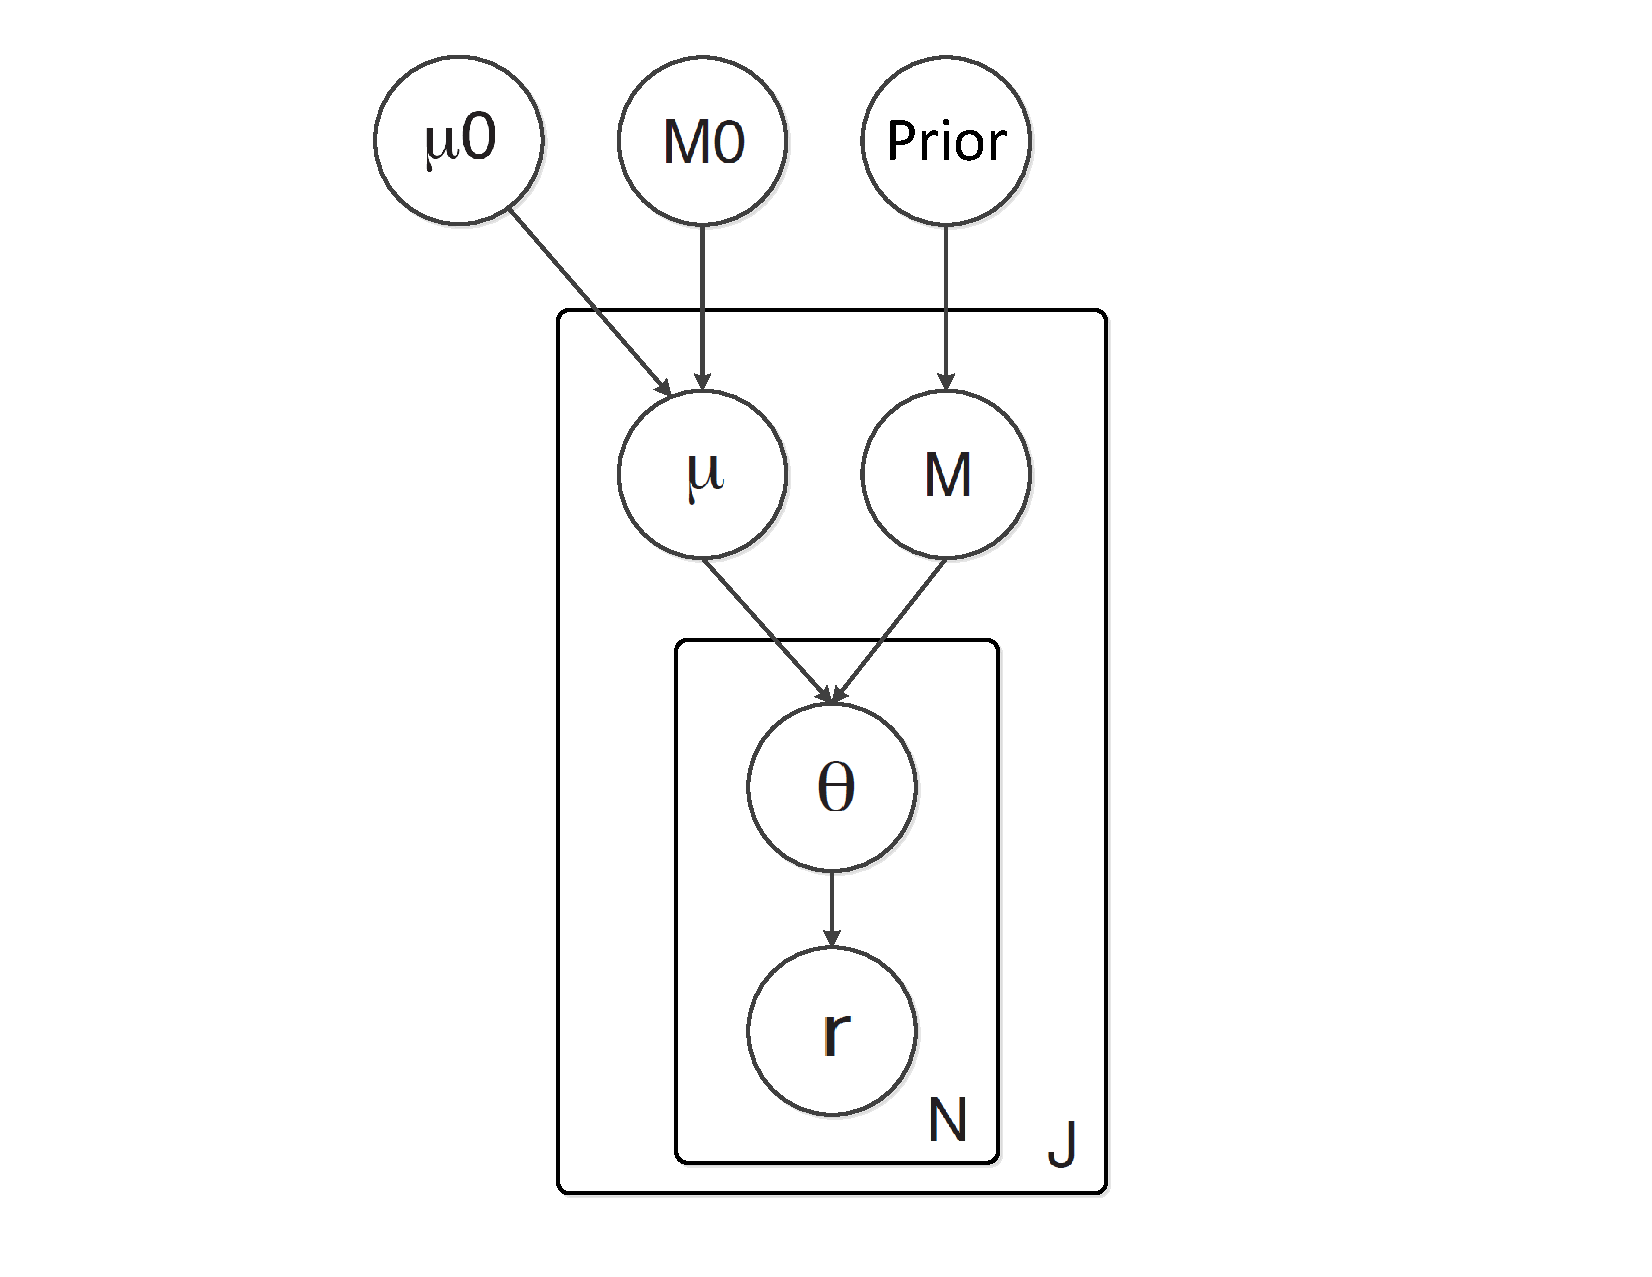
\includegraphics[width=85mm]{figs/RVD3_model.pdf}
\caption{RVD3 Graphical Model}
\label{fig:graphical_model}
\end{center}
\end{figure}


%%%%%%%%%%%%%%%%%%
% Inference & Hypothesis Testing
%%%%%%%%%%%%%%%%%%
\subsection{Inference and Hypothesis Testing}


%%%%%%%%%%%%%%%%%%%%%%%%%%
% Priors for precision parameter
%%%%%%%%%%%%%%%%%%%%%%%%%%
\subsection{Priors for precision parameter}
The prior distribution characterizes the knowledge of the parameters in the statistical model. Including prior information in the Bayesian approach is difficult but meaningful. A way to choose the prior function is to use the Schwarz criterion or Bayesian information criterion (BIC) \citep{weakliem1999critique}. Besides, the Bayes factor does tend to be more sensitive to access the prior distributions on the model parameters \citep{kass1995bayes}. To consider the Bayesian sensitivity analysis, a more practical way is to consider the range of posterior quantities of interest- the posterior mean or posterior probability \citep{bayarri1998robust, stocker2006noise, harrison2013bayesian}. Based on this theory, we analyze the posterior and prior probability of the precision hyper-parameter.
For this purpose, a bunch of different priors should be chosen for analysis \citep{gelman2006prior}. In a polygenic modeling with Bayesian sparse linear mixed model research, the results don't change dramatically by changing the prior measurement which reveals that the prior specification for the hyper-parameters are fine \citep{zhou2013polygenic}. So we performed three different plausible prior distributions: improper prior, informative prior (log-normal), and non-informative prior (Jeffrey's).

An improper prior is the prior distribution integrates to infinity, and may cause an improper posterior which results in an invalid inferences \citep{lesaffre2012bayesian}.
Furthermore when the Markov chain Monte Carlo method is taken to derive the posterior, it is possibly hard to sniff out the improper posterior.
Even though no problems happened in estimation by improper prior, other troubles could be caused in the Bayesian inference and analysis by it \citep{stein1965approximation}.
Playing no prior on $ M_{j}$ is exactly an implicit improper prior. Therefore we considered about non-informative prior and informative prior for sensitivity analysis.

Informative prior distribution is the most specific type of prior. A good informative prior is imperative to promote accurate posterior estimates.
In our study, log-normal prior is a proper prior for the beta density's parameters, $\theta_{ji} \thicksim \text{Beta}(\mu_j, M_j)$.
The parameters of it denoted $\mu$ (mean) and $\sigma$ (standard deviation) respectively.

Non-informative prior seems to be more unbiased and objective.
Various non-informative prior distributions have been suggested for parameters in hierarchical models.
Jeffrey's prior, as a typical and influential one, is proposed to establish a least informative prior that is automatically invariant to transformations by Harold Jeffreys \citep{jeffreys1946invariant}.
It is defined in terms of the Fisher information and works well with a single parameter. In our research Jeffrey's prior for $M_j$ is the square root of Fisher information of $M_j$.

%%%%%%%%%%%%%%%%%%
% Results
%%%%%%%%%%%%%%%%%%
\section{Results}

%%%%%%%%%%%%%%%%%%
% Sensitivity analysis of priors
%%%%%%%%%%%%%%%%%%
\subsection{Sensitivity analysis}

The Bayesian posterior predictive distributions and the priors distributions are shown in Figure~\ref{fig:dilu_10}.
These plots indicate the probability distribution over different M values when dilution is 10\% at $100\times$ read depth rate.
The positions are chosen in the middle of the base length- position 104 and 244 are mutant, and position 100 and 300 are non-mutant.
The posterior probability distributions are estimated by Gaussian Kernel Density \citep{silverman1986density}.
Generally the distribution plots display normal and stable without a peak nor a strange shape.
The two distributions show different ways of the prior and posterior.
The log-normal prior attributes a higher prior probability to M values between 0 and 2000.
The Jeffrey's prior assigns more information than the log-normal prior (flat) from the posterior curve.
They both want to search for a small value for M from the prior curve.

The proper prior (log-normal) and non-informative prior (Jeffrey��s) are performed to compare with the improper prior. There is little variability across positions indicating that the replication variance does not change greatly across position. We show several key parameters of the model in Figure~\ref{fig:priors_compare}. A key model parameter M is less variable with a log-normal and improper prior compared to the Jeffrey��s prior.
Additionally, the error rate across positions is captured by the $M_0$ parameter shown as a horizontal dotted line in the plots. $M_j$ is greater than $M_0$ shows that the precision between replicates is higher than the precision across positions.

\begin{figure*}[!tbp]
\begin{center}
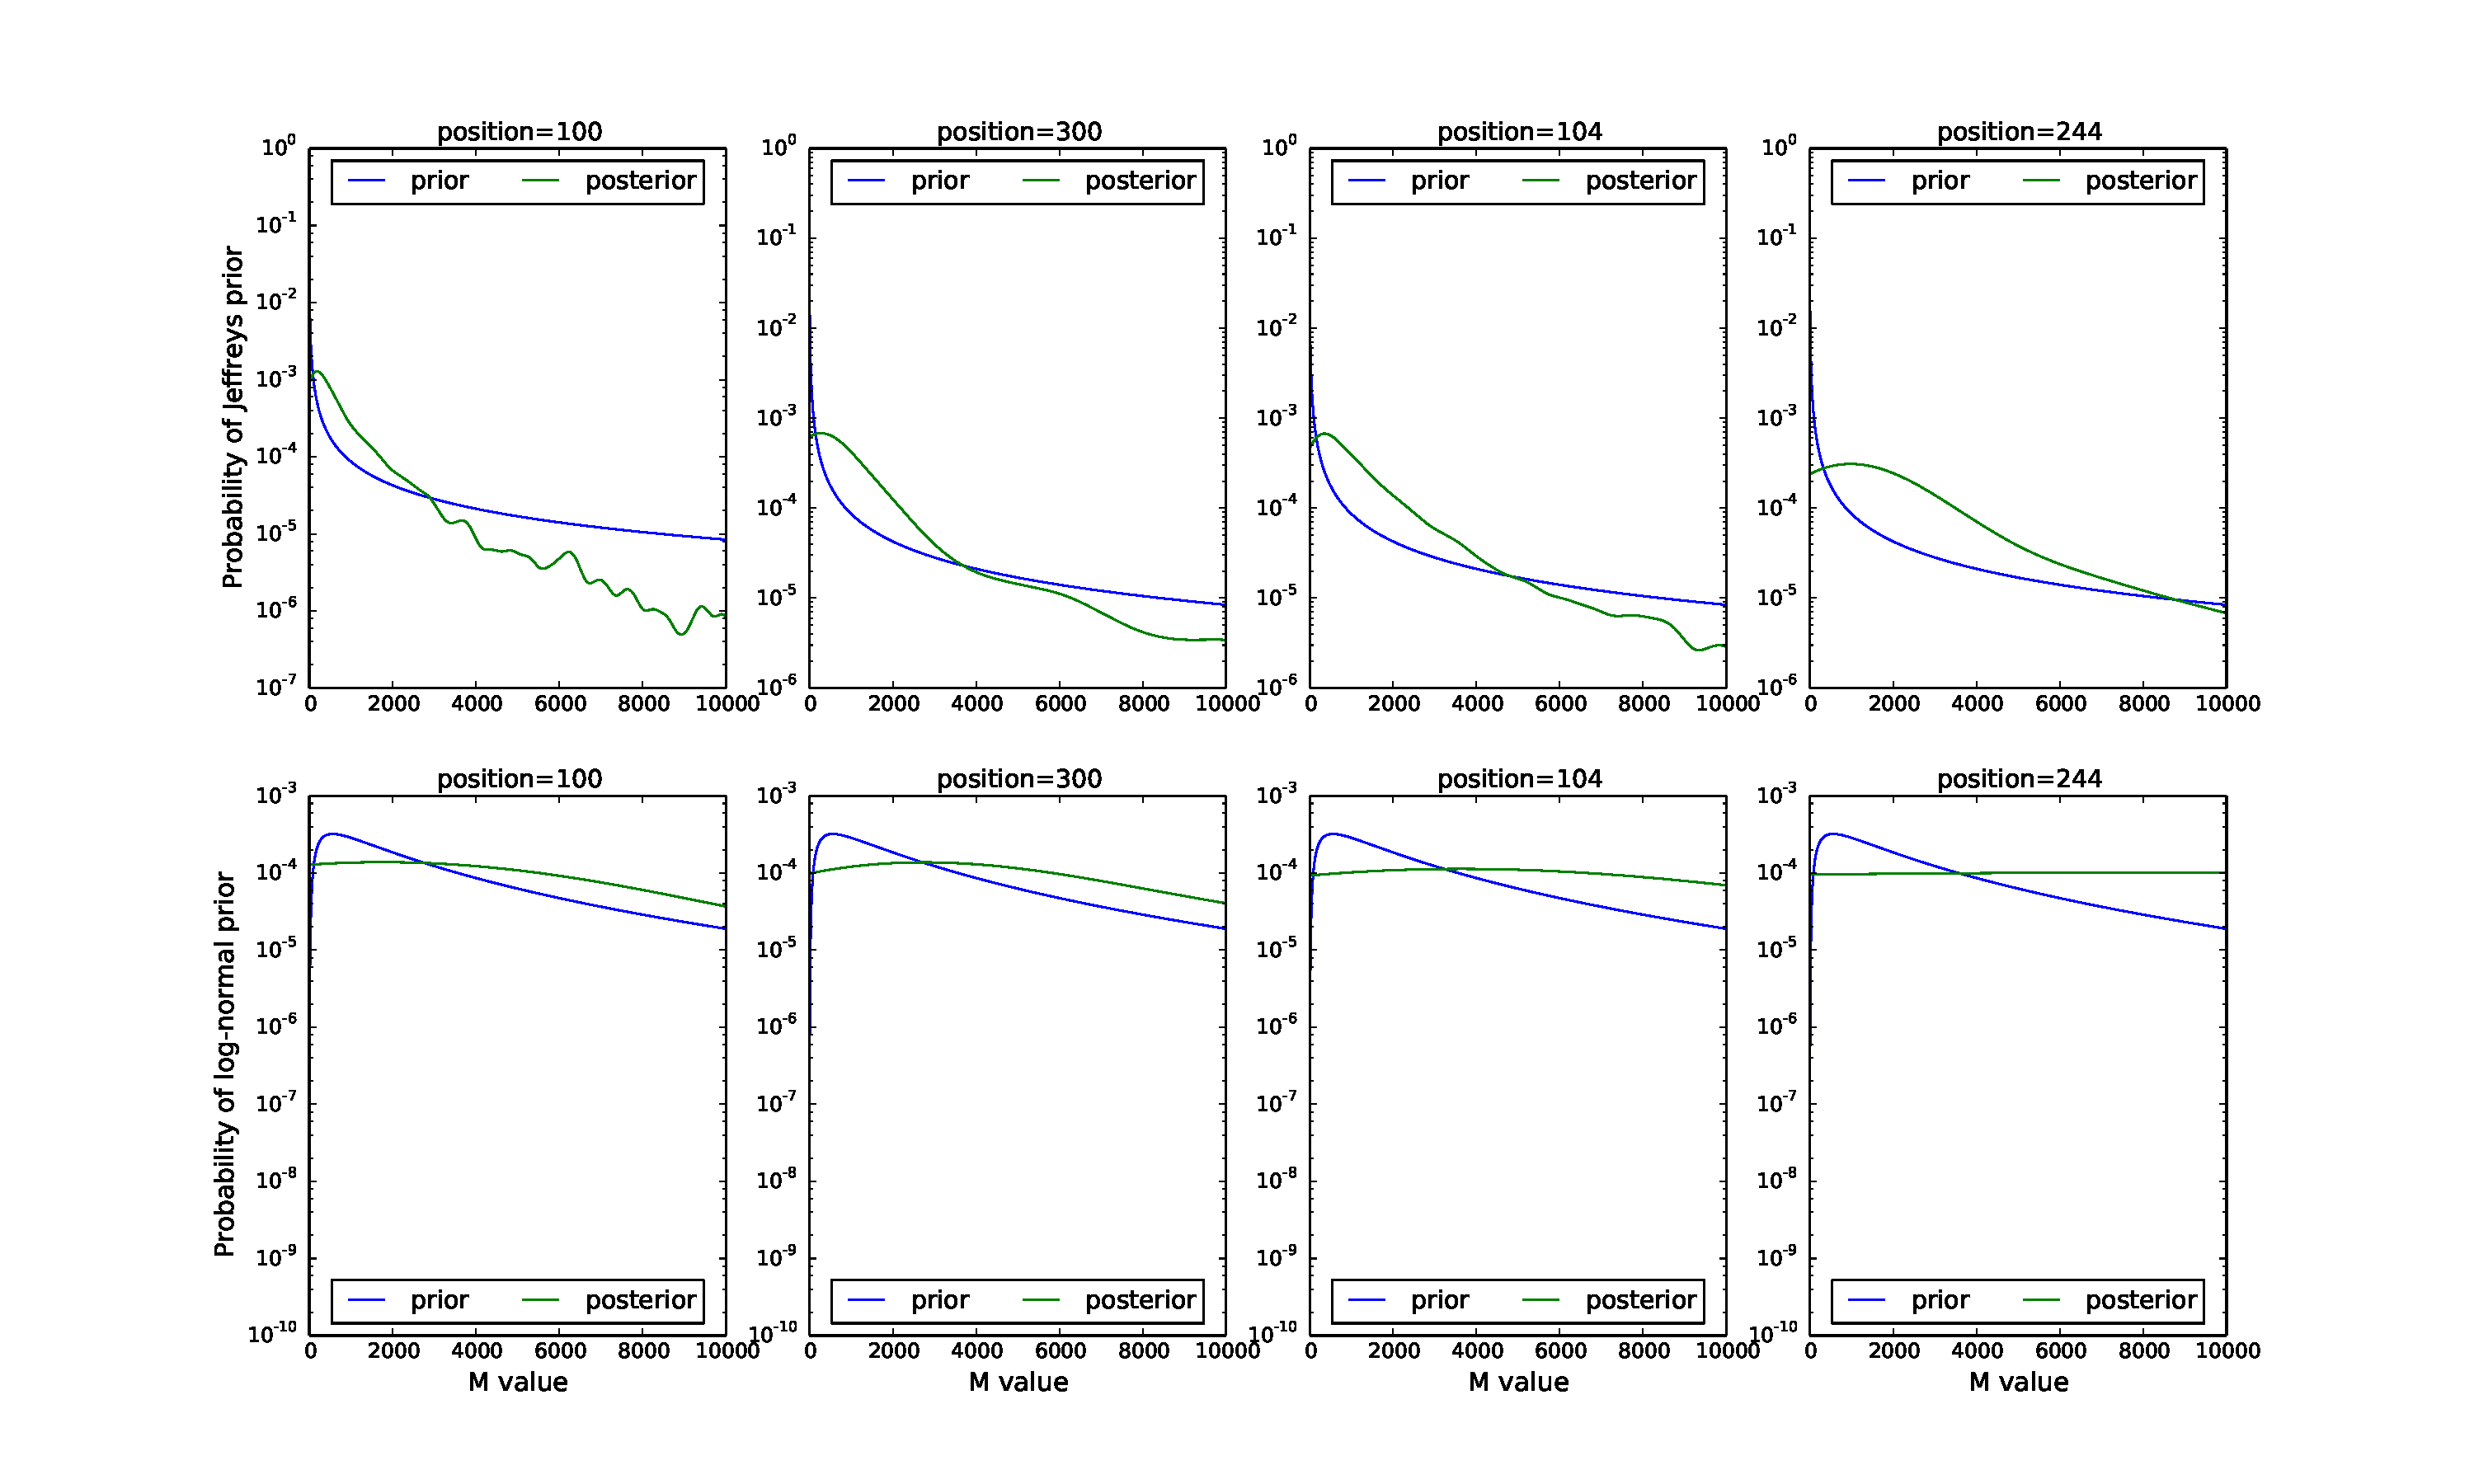
\includegraphics[width=185mm]{figs/post_prior_dilu_10.pdf}
\caption{Distribution of priors and posteriors when dilution is 10\%}
\label{fig:dilu_10}
\end{center}
\end{figure*}

\begin{figure}[htbp]
\begin{center}
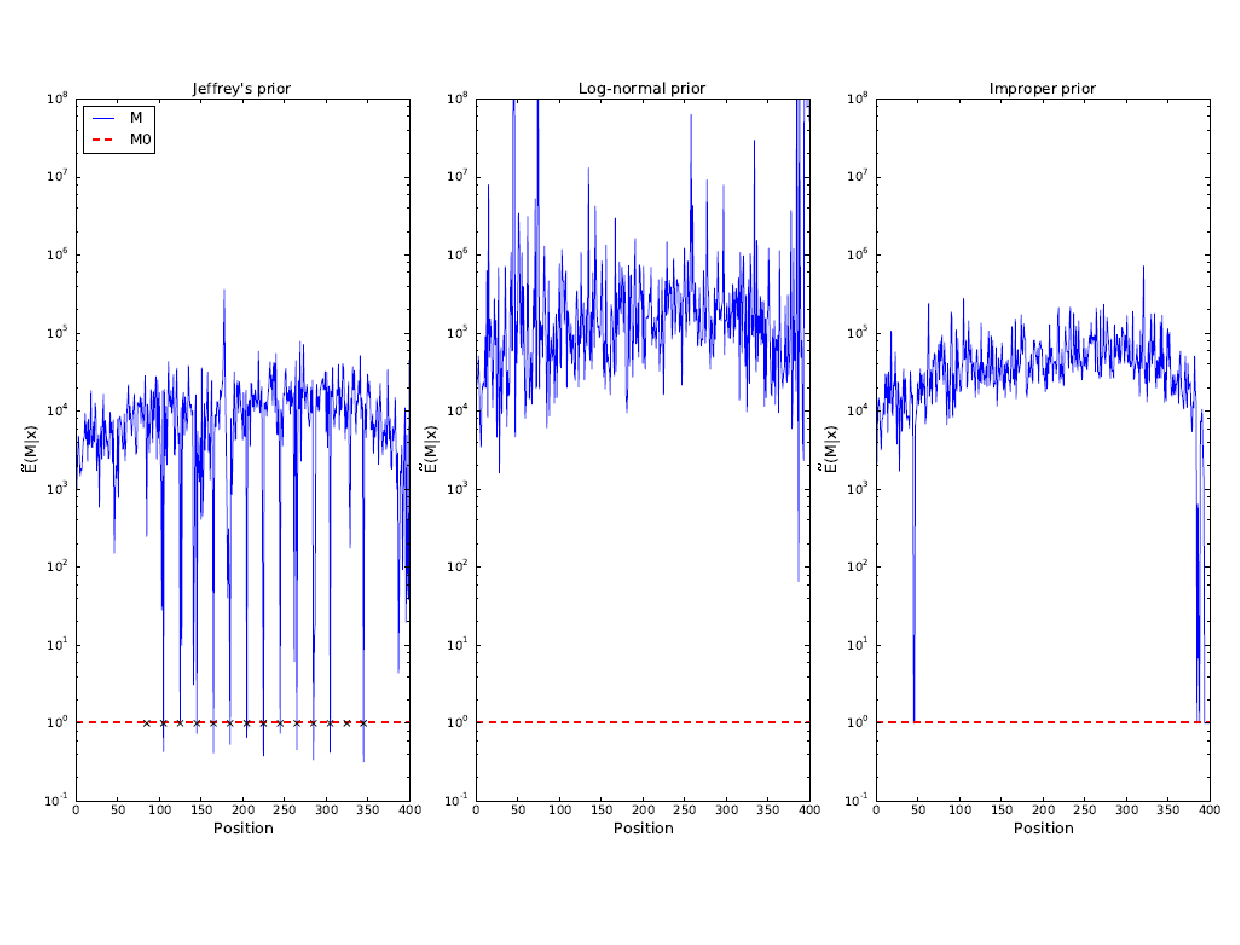
\includegraphics[width=160mm]{figs/priors_compare.pdf}
\caption{Key parameters for RVD3 model with different priors.}
\label{fig:priors_compare}
\end{center}
\end{figure}

%%%%%%%%%%%%%%%%%%%%%%%%%%%%%
% Results of priors on synthetic data
%%%%%%%%%%%%%%%%%%%%%%%%%%%%%
\subsection{Results of priors on synthetic data}
The RVD3 model is analyzed by the selecting two reasonable prior distributions, and the corresponding results are compared from the aspects of performance with different read depths, sensitivity and specificity, and FDR.

\subsubsection{Performance with read depth}

\begin{figure}[htbp]
\begin{center}
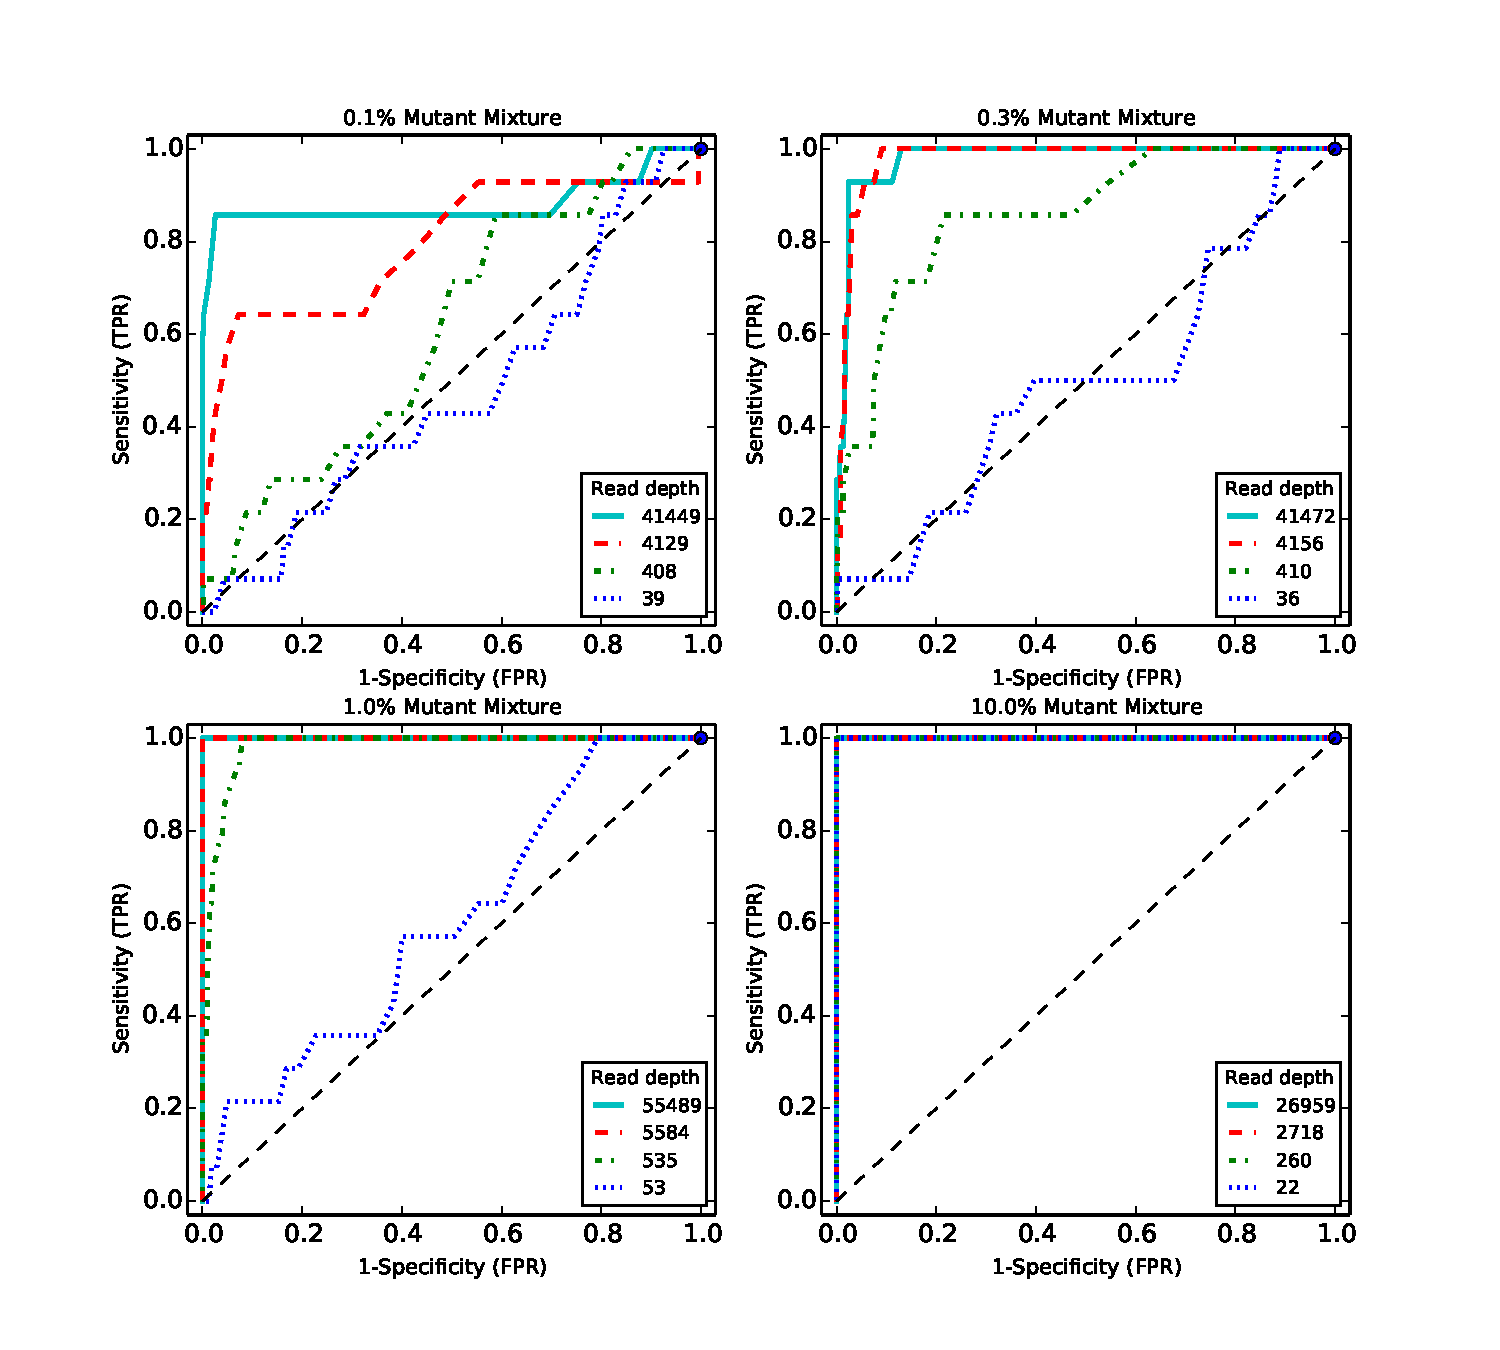
\includegraphics[width=90mm]{figs/ROC_without_chi2_jeffrey.pdf}
\caption{ROC curve for variants detection performance by Jeffrey's prior.}
\label{fig:ROC_jeffrey}
\end{center}
\end{figure}

\begin{figure}[htbp]
\begin{center}
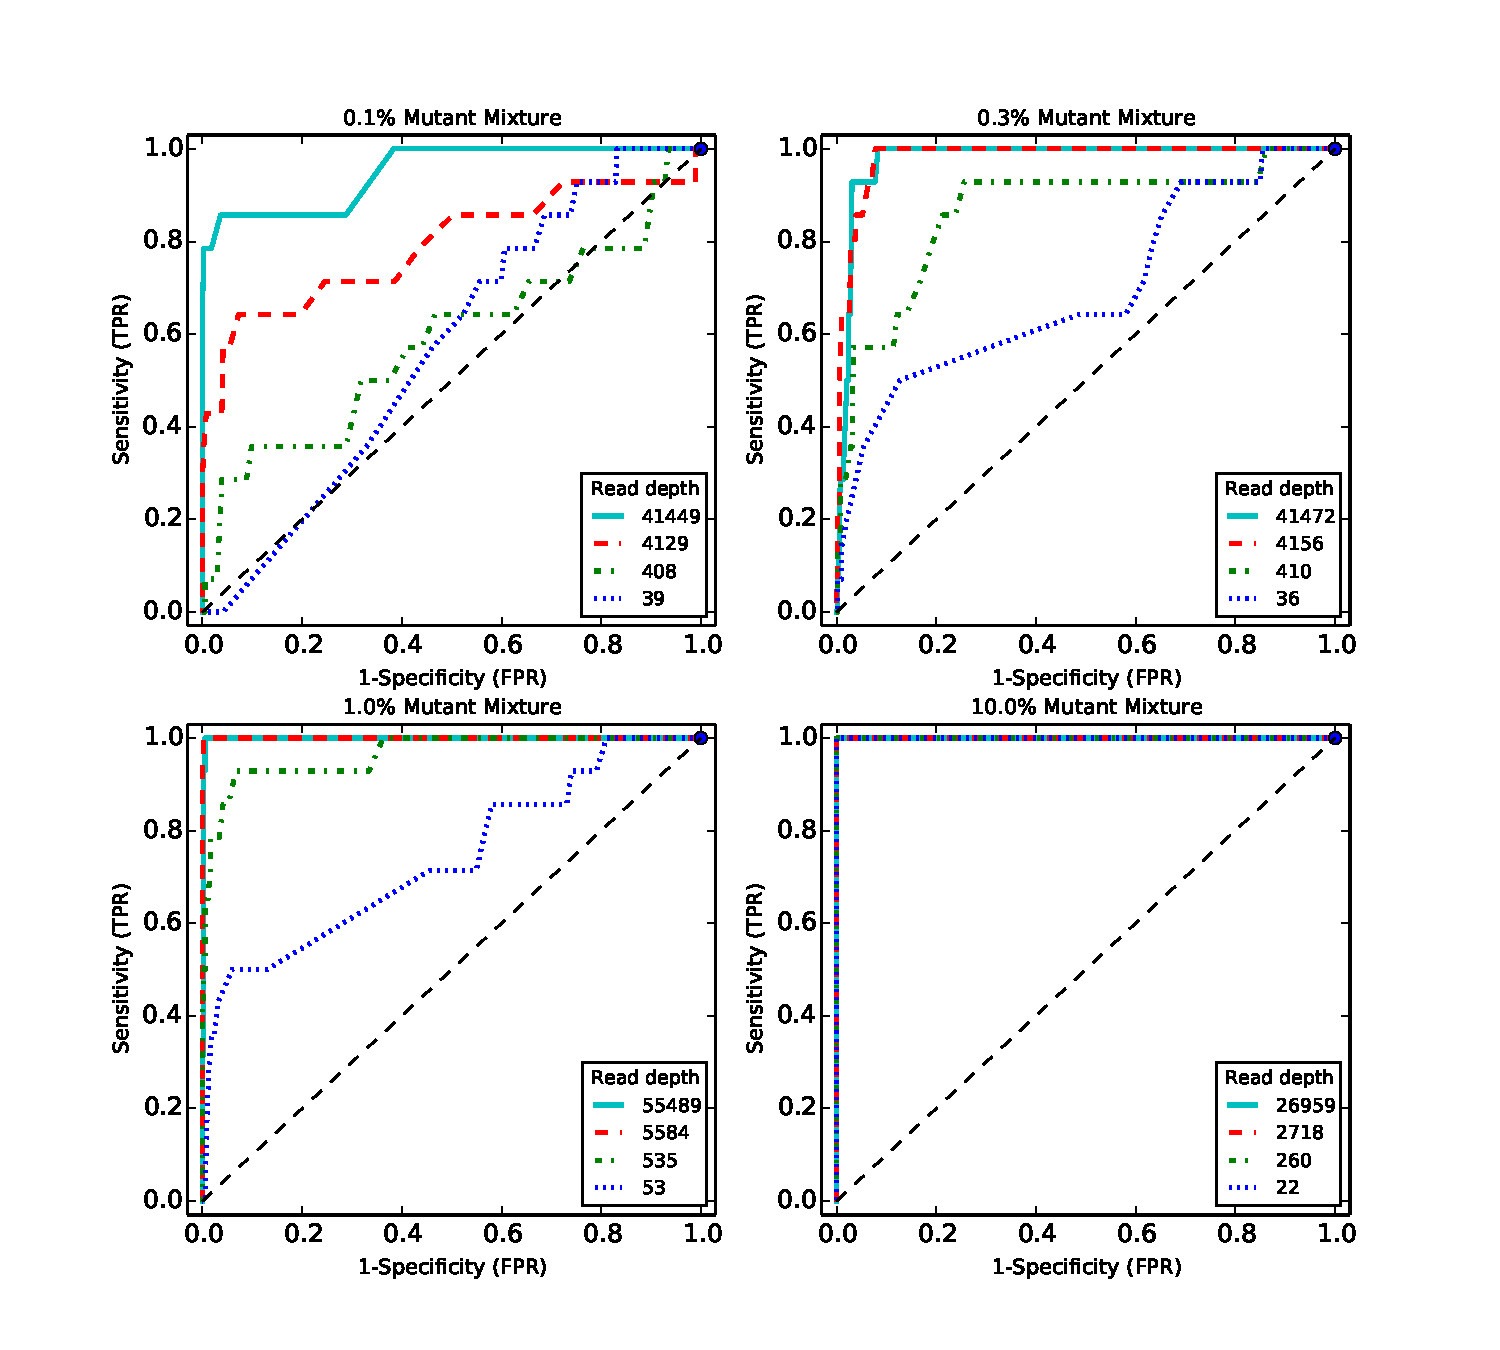
\includegraphics[width=90mm]{figs/ROC_without_chi2_lognormal.pdf}
\caption{ROC curve for variants detection performance by log-normal prior.}
\label{fig:ROC_lognormal}
\end{center}
\end{figure}


To evaluate the performance of RVD3 model with priors, we generated receiver-operating characteristic curves (ROCs) for median read depth and minor allele frequencies (MAFs).
Here the Bayesian test is used without the $\chi^2$ test. Figure~\ref{fig:ROC_jeffrey} and Figure~\ref{fig:ROC_lognormal} shows ROC curves with a fixed $\alpha=0.05$.
The performance improves when the read depth goes up. (ROC shows that the model with priors performs better than improper prior situation especially on the small read depth).
Noticed at the lowest depth (22) with 10.0\% mutant mixture, the sensitivity and specificity value are 1 and much better than the model with improper priors for $M_j$, which definitely demonstrates the advantage of priors.

\subsubsection{Sensitivity/Specificity/FDR}

Figure~\ref{fig:SS} shows that the sensitivity and specificity of the RVD3 of different priors compared with the model with improper priors.
Log-normal prior shows a higher sensitivity and specificity value than the Jeffrey's prior.
Figure~\ref{fid:fdr} shows the false discovery rate of the RVD3 with different priors. Jeffrey's prior shows a smaller false discovery rate than others.
It is obvious no matter Jeffrey's or log-normal prior, the variant detection performance acquires lower FDR to a known 0.1\% minor allele frequency event, compared with improper priors, which seems desirable of our model for extending for a broad application.
Based on the various advantages for Jeffrey's and log-normal prior, RVD3 can afford a more appropriate choice for the precision parameter.
Here we chose Jeffrey's prior model because it's a non-informative prior, and more attention should be paid to false discovery rate and accuracy for variants calling research, compared with the clinical experiment or diagnosis which cares more on true positive rate and true negative rate.


\begin{figure}[htbp]
\begin{center}
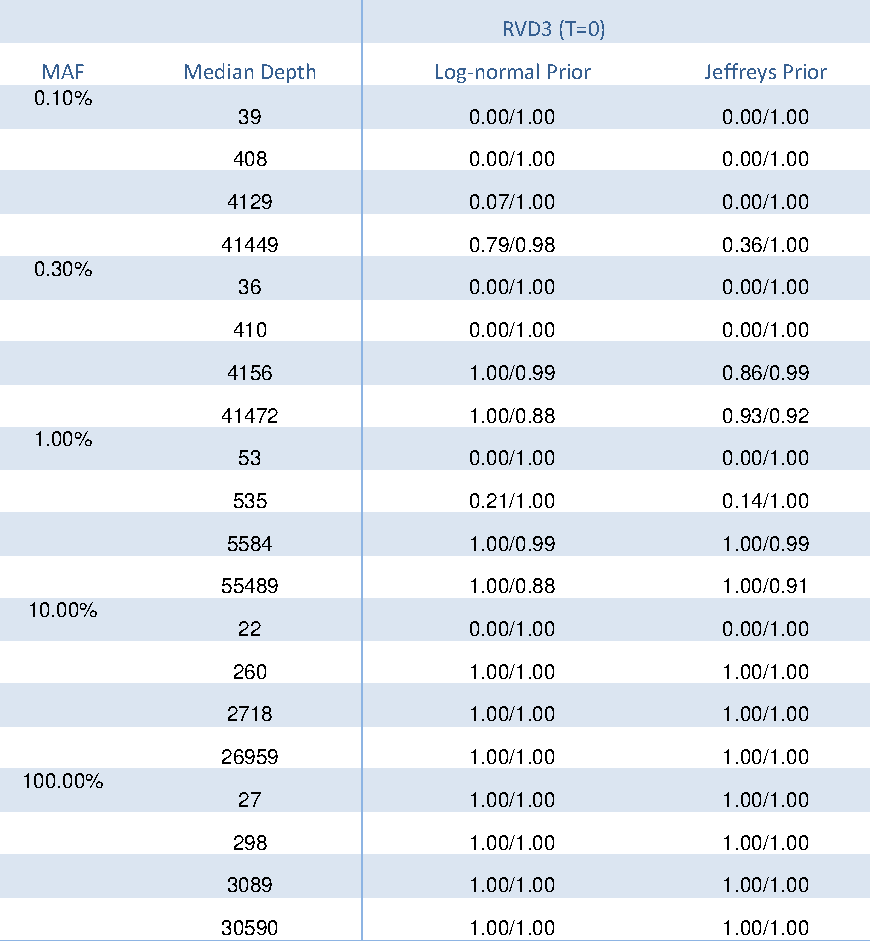
\includegraphics[width=80mm]{tables/Sen_Speci.pdf}
\caption{Sensitivity/Specificity comparison of RVD3 with different priors.}
\label{fig:SS}
\end{center}
\end{figure}


\begin{figure}[htbp]
\begin{center}
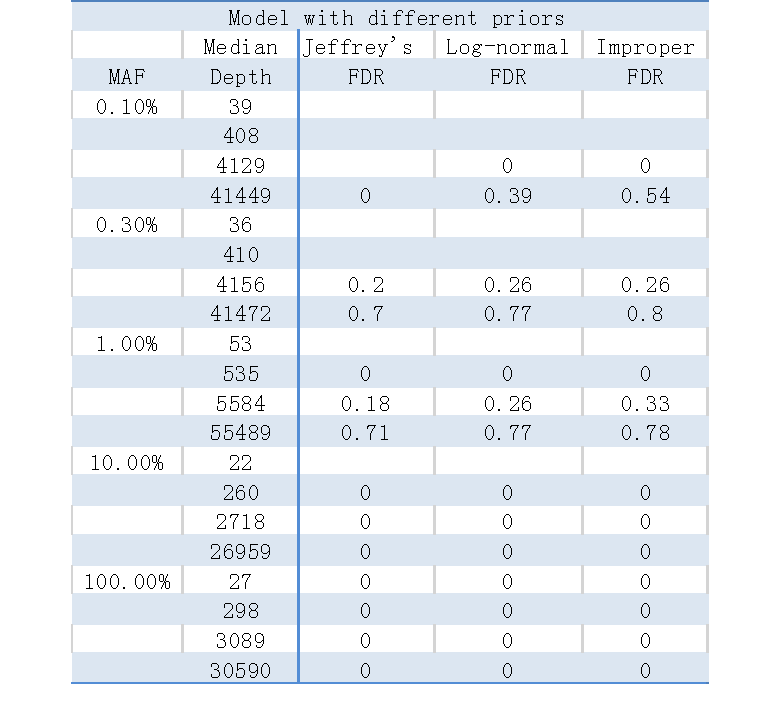
\includegraphics[width=80mm]{tables/FDR.pdf}
\caption{False Discovery Rate comparison with different priors on RVD3.}
\label{fig:fdr}
\end{center}
\end{figure}

%%%%%%%%%%%%%%%%%%%%%%%%%%%%%%
% Results of Jeffrey's prior on yeast data
%%%%%%%%%%%%%%%%%%%%%%%%%%%%%%
\subsection{Results of Jeffrey's prior on yeast data}

We demonstrated our RVD3 model with Jeffrey's prior on yeast data to identify the variants \citep{kvitek2013whole}.


\section{Discussion}


\section{Conclusion}


\appendix
%%%%%%%%%%%%%%%%%%%
% Appendix A: Parameter Initialization
%%%%%%%%%%%%%%%%%%%
\section{Parameter Initialization}\label{sec:appendix_mom}
[This part is COPIED]

Since $r_{ji} \thicksim \text{Binomial}(n_{ji}, \theta_{ji})$, the first population moment is  $E[r_{ji}] = \theta_{ji} n_{ji}$ and the first sample moment is simply $m_1 = r_{ji}$.
Therefore the MoM estimator is
\begin{equation}
	\tilde{\theta}_{ji} = \frac{r_{ji}} {n_{ji}}
\end{equation}

We take the MoM estimate, $\tilde{\theta}_{ji}$, as data for the next conditional distribution in the hierarchical model.
The distribution is $\theta_{ji} \thicksim \text{Beta}(\mu_jM_j, (1-\mu_j)M_j)$. The first and second population moments are
\begin{eqnarray}
	E[\theta_{ji}] =& \mu_j,\\
	\text{Var}[\theta_{ji}] =& \frac{\mu_j(1-\mu_j)} { M_j + 1 }.
\end{eqnarray}
The first and second sample moments are $m_1 = \frac{1}{N}\sum_{i=1}^N \theta_{ji}$ and $m_2 = \frac{1}{N}\sum_{i=1}^N \theta_{ji}^2$.
Setting the population moments equal to the sample moments and solving for $\mu_j$ and $M_j$ gives
\begin{eqnarray}
	\tilde{\mu}_j =& \frac{1}{N} \sum_{i=1}^N \theta_{ji}, \\
	\tilde{M_j} =& \frac{ \tilde{\mu}_j (1 - \tilde{\mu}_j ) } { \frac{1}{N} \sum_{i=1}^N \theta_{ji}^2 } -1.
\end{eqnarray}

Following the same procedure for the parameters of $\mu_j \thicksim \text{Beta}(\mu_0, M_0)$ gives the following MoM estimates
\begin{eqnarray}
	\tilde{\mu}_0 =& \frac{1}{J} \sum_{j=1}^J \mu_j \\
	\tilde{M}_0 =& \frac{ \tilde{\mu}_0 (1 - \tilde{\mu}_0 ) } {\frac{1}{J} \sum_{j=1}^J \mu_j^2 } -1.
\end{eqnarray}

%%%%%%%%%%%%%%%%%%%
% Appendix B: Inference of Jeffreys prior
%%%%%%%%%%%%%%%%%%%
\section{Inference of Jeffrey's prior}\label{sec:appendix_Jeffreys}
We assume there is only one replicate (i=1),

\begin{equation}\label{eqn:Betapdf}
p\left({\theta }_{j} \right)= \frac{\Gamma \left({M}_{j} \right)}{\Gamma \left({\mu }_{j} {M}_{j}\right)\Gamma \left(( 1-{\mu }_{j}){M}_{j}\right)} {{\theta}_{j}}^{{\mu}_{j}{M}_{j}-1}{\left(1-\theta\right)_{j}}^{\left(1-{\mu}_{j}\right){M}_{j}-1}
\end{equation}

\begin{equation}\label{equ:JefferyInference1}
\begin{split}
&\log p\left(\theta_{j}|\mu_{j},M_{j}\right) =\log \Gamma \left(M_{j}\right)-\log \Gamma\left(\mu_{j},M_{j}\right)\\
&- \log \Gamma\left(1-\mu_{j},M_{j}\right) + (\mu_{j}M_{j}-1)\log\theta_{j}\\
& + ((1-\,u_{j})M_{j}-1)\log(1-\theta_{j})\
\end{split}
\end{equation}

\begin{equation}
\begin{split}
&\frac{\delta\log p(\theta_{j})}{\delta M_{j}} =\Psi(M_{j}) - \Psi(\mu_{j} M_{j})\mu_{j}\\
&- \Psi((1-\mu_{j})M_{j})(1-\mu_{j}) +\mu_{j}\log\theta_{j} + (1-\mu_{j})\log(1-\theta_{j})\
\end{split}
\end{equation}

\begin{equation}
\frac{\delta^{2}\log p(\theta_{j})}{\delta M_{j}^{2}}  = \Psi_{1}(M_{j}) - \Psi_{1}(\mu_{j} M_{j})\mu_{j}^{2} - \Psi_{1}((1-\mu_{j})M_{j})(1-\mu_{j})^{2}
\end{equation}

Now we have the Jeffreys' prior $\pi\left({M}_{j}\right)$ for $M_{j}$:

\begin{equation}
[-\left(\Psi_{1}(M_{j}) - \Psi_{1}(\mu_{j} M_{j})\mu_{j}^{2} - \Psi_{1}((1-\mu_{j})M_{j}){(1-\mu_{j})^{2}}\right)]^{\frac{1}{2}}
\end{equation}


\bibliographystyle{apalike}
\bibliography{bioinfo}
\end{document}
